\documentclass[]{thesis-ekf}
\usepackage[T1]{fontenc}
\PassOptionsToPackage{defaults=hu-min}{magyar.ldf}
\usepackage[magyar]{babel}
\usepackage{mathtools,amssymb,amsthm,pdfpages,listings,multicol,enumitem,wrapfig}
\footnotestyle{rule=fourth}

\newtheorem{tetel}{Tétel}[chapter]
\theoremstyle{definition}
\newtheorem{definicio}[tetel]{Definíció}
\theoremstyle{remark}
\newtheorem{megjegyzes}[tetel]{Megjegyzés}
 %%%%%%%%%%%%%%%%%%%%%%%%%%%%%%%%%%%%%%%%%%%%%%%%%%%%%%%%%%%%%%%%%%%%%%%%%%%%%%%% 
%%% ~ Arduino Language - Arduino IDE Colors ~                                  %%%
%%%                                                                            %%%
%%% Kyle Rocha-Brownell | 10/2/2017 | No Licence                               %%%
%%% -------------------------------------------------------------------------- %%%
%%%                                                                            %%%
%%% Place this file in your working directory (next to the latex file you're   %%%
%%% working on).  To add it to your project, place:                            %%%
%%%     %%%%%%%%%%%%%%%%%%%%%%%%%%%%%%%%%%%%%%%%%%%%%%%%%%%%%%%%%%%%%%%%%%%%%%%%%%%%%%%% 
%%% ~ Arduino Language - Arduino IDE Colors ~                                  %%%
%%%                                                                            %%%
%%% Kyle Rocha-Brownell | 10/2/2017 | No Licence                               %%%
%%% -------------------------------------------------------------------------- %%%
%%%                                                                            %%%
%%% Place this file in your working directory (next to the latex file you're   %%%
%%% working on).  To add it to your project, place:                            %%%
%%%     %%%%%%%%%%%%%%%%%%%%%%%%%%%%%%%%%%%%%%%%%%%%%%%%%%%%%%%%%%%%%%%%%%%%%%%%%%%%%%%% 
%%% ~ Arduino Language - Arduino IDE Colors ~                                  %%%
%%%                                                                            %%%
%%% Kyle Rocha-Brownell | 10/2/2017 | No Licence                               %%%
%%% -------------------------------------------------------------------------- %%%
%%%                                                                            %%%
%%% Place this file in your working directory (next to the latex file you're   %%%
%%% working on).  To add it to your project, place:                            %%%
%%%    \input{arduinoLanguage.tex}                                             %%%
%%% somewhere before \begin{document} in your latex file.                      %%%
%%%                                                                            %%%
%%% In your document, place your arduino code between:                         %%%
%%%   \begin{lstlisting}[language=Arduino]                                     %%%
%%% and:                                                                       %%%
%%%   \end{lstlisting}                                                         %%%
%%%                                                                            %%%
%%% Or create your own style to add non-built-in functions and variables.      %%%
%%%                                                                            %%%
 %%%%%%%%%%%%%%%%%%%%%%%%%%%%%%%%%%%%%%%%%%%%%%%%%%%%%%%%%%%%%%%%%%%%%%%%%%%%%%%% 

\usepackage{color}
\usepackage{listings}    
\usepackage{courier}

%%% Define Custom IDE Colors %%%
\definecolor{arduinoGreen}    {rgb} {0.17, 0.43, 0.01}
\definecolor{arduinoGrey}     {rgb} {0.47, 0.47, 0.33}
\definecolor{arduinoOrange}   {rgb} {0.8 , 0.4 , 0   }
\definecolor{arduinoBlue}     {rgb} {0.01, 0.61, 0.98}
\definecolor{arduinoDarkBlue} {rgb} {0.0 , 0.2 , 0.5 }

%%% Define Arduino Language %%%
\lstdefinelanguage{Arduino}{
  language=C++, % begin with default C++ settings 
%
%
  %%% Keyword Color Group 1 %%%  (called KEYWORD3 by arduino)
  keywordstyle=\color{arduinoGreen},   
  deletekeywords={  % remove all arduino keywords that might be in c++
                break, case, override, final, continue, default, do, else, for, 
                if, return, goto, switch, throw, try, while, setup, loop, export, 
                not, or, and, xor, include, define, elif, else, error, if, ifdef, 
                ifndef, pragma, warning,
                HIGH, LOW, INPUT, INPUT_PULLUP, OUTPUT, DEC, BIN, HEX, OCT, PI, 
                HALF_PI, TWO_PI, LSBFIRST, MSBFIRST, CHANGE, FALLING, RISING, 
                DEFAULT, EXTERNAL, INTERNAL, INTERNAL1V1, INTERNAL2V56, LED_BUILTIN, 
                LED_BUILTIN_RX, LED_BUILTIN_TX, DIGITAL_MESSAGE, FIRMATA_STRING, 
                ANALOG_MESSAGE, REPORT_DIGITAL, REPORT_ANALOG, SET_PIN_MODE, 
                SYSTEM_RESET, SYSEX_START, auto, int8_t, int16_t, int32_t, int64_t, 
                uint8_t, uint16_t, uint32_t, uint64_t, char16_t, char32_t, operator, 
                enum, delete, bool, boolean, byte, char, const, false, float, double, 
                null, NULL, int, long, new, private, protected, public, short, 
                signed, static, volatile, String, void, true, unsigned, word, array, 
                sizeof, dynamic_cast, typedef, const_cast, struct, static_cast, union, 
                friend, extern, class, reinterpret_cast, register, explicit, inline, 
                _Bool, complex, _Complex, _Imaginary, atomic_bool, atomic_char, 
                atomic_schar, atomic_uchar, atomic_short, atomic_ushort, atomic_int, 
                atomic_uint, atomic_long, atomic_ulong, atomic_llong, atomic_ullong, 
                virtual, PROGMEM,
                Serial, Serial1, Serial2, Serial3, SerialUSB, Keyboard, Mouse,
                abs, acos, asin, atan, atan2, ceil, constrain, cos, degrees, exp, 
                floor, log, map, max, min, radians, random, randomSeed, round, sin, 
                sq, sqrt, tan, pow, bitRead, bitWrite, bitSet, bitClear, bit, 
                highByte, lowByte, analogReference, analogRead, 
                analogReadResolution, analogWrite, analogWriteResolution, 
                attachInterrupt, detachInterrupt, digitalPinToInterrupt, delay, 
                delayMicroseconds, digitalWrite, digitalRead, interrupts, millis, 
                micros, noInterrupts, noTone, pinMode, pulseIn, pulseInLong, shiftIn, 
                shiftOut, tone, yield, Stream, begin, end, peek, read, print, 
                println, available, availableForWrite, flush, setTimeout, find, 
                findUntil, parseInt, parseFloat, readBytes, readBytesUntil, readString, 
                readStringUntil, trim, toUpperCase, toLowerCase, charAt, compareTo, 
                concat, endsWith, startsWith, equals, equalsIgnoreCase, getBytes, 
                indexOf, lastIndexOf, length, replace, setCharAt, substring, 
                toCharArray, toInt, press, release, releaseAll, accept, click, move, 
                isPressed, isAlphaNumeric, isAlpha, isAscii, isWhitespace, isControl, 
                isDigit, isGraph, isLowerCase, isPrintable, isPunct, isSpace, 
                isUpperCase, isHexadecimalDigit, 
                }, 
  morekeywords={   % add arduino structures to group 1
                break, case, override, final, continue, default, do, else, for, 
                if, return, goto, switch, throw, try, while, setup, loop, export, 
                not, or, and, xor, include, define, elif, else, error, if, ifdef, 
                ifndef, pragma, warning,
                }, 
% 
%
  %%% Keyword Color Group 2 %%%  (called LITERAL1 by arduino)
  keywordstyle=[2]\color{arduinoBlue},   
  keywords=[2]{   % add variables and dataTypes as 2nd group  
                HIGH, LOW, INPUT, INPUT_PULLUP, OUTPUT, DEC, BIN, HEX, OCT, PI, 
                HALF_PI, TWO_PI, LSBFIRST, MSBFIRST, CHANGE, FALLING, RISING, 
                DEFAULT, EXTERNAL, INTERNAL, INTERNAL1V1, INTERNAL2V56, LED_BUILTIN, 
                LED_BUILTIN_RX, LED_BUILTIN_TX, DIGITAL_MESSAGE, FIRMATA_STRING, 
                ANALOG_MESSAGE, REPORT_DIGITAL, REPORT_ANALOG, SET_PIN_MODE, 
                SYSTEM_RESET, SYSEX_START, auto, int8_t, int16_t, int32_t, int64_t, 
                uint8_t, uint16_t, uint32_t, uint64_t, char16_t, char32_t, operator, 
                enum, delete, bool, boolean, byte, char, const, false, float, double, 
                null, NULL, int, long, new, private, protected, public, short, 
                signed, static, volatile, String, void, true, unsigned, word, array, 
                sizeof, dynamic_cast, typedef, const_cast, struct, static_cast, union, 
                friend, extern, class, reinterpret_cast, register, explicit, inline, 
                _Bool, complex, _Complex, _Imaginary, atomic_bool, atomic_char, 
                atomic_schar, atomic_uchar, atomic_short, atomic_ushort, atomic_int, 
                atomic_uint, atomic_long, atomic_ulong, atomic_llong, atomic_ullong, 
                virtual, PROGMEM,
                },  
% 
%
  %%% Keyword Color Group 3 %%%  (called KEYWORD1 by arduino)
  keywordstyle=[3]\bfseries\color{arduinoOrange},
  keywords=[3]{  % add built-in functions as a 3rd group
                Serial, Serial1, Serial2, Serial3, SerialUSB, Keyboard, Mouse,
                },      
%
%
  %%% Keyword Color Group 4 %%%  (called KEYWORD2 by arduino)
  keywordstyle=[4]\color{arduinoOrange},
  keywords=[4]{  % add more built-in functions as a 4th group
                abs, acos, asin, atan, atan2, ceil, constrain, cos, degrees, exp, 
                floor, log, map, max, min, radians, random, randomSeed, round, sin, 
                sq, sqrt, tan, pow, bitRead, bitWrite, bitSet, bitClear, bit, 
                highByte, lowByte, analogReference, analogRead, 
                analogReadResolution, analogWrite, analogWriteResolution, 
                attachInterrupt, detachInterrupt, digitalPinToInterrupt, delay, 
                delayMicroseconds, digitalWrite, digitalRead, interrupts, millis, 
                micros, noInterrupts, noTone, pinMode, pulseIn, pulseInLong, shiftIn, 
                shiftOut, tone, yield, Stream, begin, end, peek, read, print, 
                println, available, availableForWrite, flush, setTimeout, find, 
                findUntil, parseInt, parseFloat, readBytes, readBytesUntil, readString, 
                readStringUntil, trim, toUpperCase, toLowerCase, charAt, compareTo, 
                concat, endsWith, startsWith, equals, equalsIgnoreCase, getBytes, 
                indexOf, lastIndexOf, length, replace, setCharAt, substring, 
                toCharArray, toInt, press, release, releaseAll, accept, click, move, 
                isPressed, isAlphaNumeric, isAlpha, isAscii, isWhitespace, isControl, 
                isDigit, isGraph, isLowerCase, isPrintable, isPunct, isSpace, 
                isUpperCase, isHexadecimalDigit,
                adns_write_reg,adns_com_begin,SPI,transfer,adns_com_end
                },      
%
%
  %%% Set Other Colors %%%
  stringstyle=\color{arduinoDarkBlue},    
  commentstyle=\color{arduinoGrey},    
%          
%   
  %%%% Line Numbering %%%%
  numbers=left,                    
  numbersep=5pt,                   
  numberstyle=\color{arduinoGrey},    
  %stepnumber=2,                      % show every 2 line numbers
%
%
  %%%% Code Box Style %%%%
  breaklines=true,                    % wordwrapping
  tabsize=2,         
  basicstyle=\ttfamily  
}
                                             %%%
%%% somewhere before \begin{document} in your latex file.                      %%%
%%%                                                                            %%%
%%% In your document, place your arduino code between:                         %%%
%%%   \begin{lstlisting}[language=Arduino]                                     %%%
%%% and:                                                                       %%%
%%%   \end{lstlisting}                                                         %%%
%%%                                                                            %%%
%%% Or create your own style to add non-built-in functions and variables.      %%%
%%%                                                                            %%%
 %%%%%%%%%%%%%%%%%%%%%%%%%%%%%%%%%%%%%%%%%%%%%%%%%%%%%%%%%%%%%%%%%%%%%%%%%%%%%%%% 

\usepackage{color}
\usepackage{listings}    
\usepackage{courier}

%%% Define Custom IDE Colors %%%
\definecolor{arduinoGreen}    {rgb} {0.17, 0.43, 0.01}
\definecolor{arduinoGrey}     {rgb} {0.47, 0.47, 0.33}
\definecolor{arduinoOrange}   {rgb} {0.8 , 0.4 , 0   }
\definecolor{arduinoBlue}     {rgb} {0.01, 0.61, 0.98}
\definecolor{arduinoDarkBlue} {rgb} {0.0 , 0.2 , 0.5 }

%%% Define Arduino Language %%%
\lstdefinelanguage{Arduino}{
  language=C++, % begin with default C++ settings 
%
%
  %%% Keyword Color Group 1 %%%  (called KEYWORD3 by arduino)
  keywordstyle=\color{arduinoGreen},   
  deletekeywords={  % remove all arduino keywords that might be in c++
                break, case, override, final, continue, default, do, else, for, 
                if, return, goto, switch, throw, try, while, setup, loop, export, 
                not, or, and, xor, include, define, elif, else, error, if, ifdef, 
                ifndef, pragma, warning,
                HIGH, LOW, INPUT, INPUT_PULLUP, OUTPUT, DEC, BIN, HEX, OCT, PI, 
                HALF_PI, TWO_PI, LSBFIRST, MSBFIRST, CHANGE, FALLING, RISING, 
                DEFAULT, EXTERNAL, INTERNAL, INTERNAL1V1, INTERNAL2V56, LED_BUILTIN, 
                LED_BUILTIN_RX, LED_BUILTIN_TX, DIGITAL_MESSAGE, FIRMATA_STRING, 
                ANALOG_MESSAGE, REPORT_DIGITAL, REPORT_ANALOG, SET_PIN_MODE, 
                SYSTEM_RESET, SYSEX_START, auto, int8_t, int16_t, int32_t, int64_t, 
                uint8_t, uint16_t, uint32_t, uint64_t, char16_t, char32_t, operator, 
                enum, delete, bool, boolean, byte, char, const, false, float, double, 
                null, NULL, int, long, new, private, protected, public, short, 
                signed, static, volatile, String, void, true, unsigned, word, array, 
                sizeof, dynamic_cast, typedef, const_cast, struct, static_cast, union, 
                friend, extern, class, reinterpret_cast, register, explicit, inline, 
                _Bool, complex, _Complex, _Imaginary, atomic_bool, atomic_char, 
                atomic_schar, atomic_uchar, atomic_short, atomic_ushort, atomic_int, 
                atomic_uint, atomic_long, atomic_ulong, atomic_llong, atomic_ullong, 
                virtual, PROGMEM,
                Serial, Serial1, Serial2, Serial3, SerialUSB, Keyboard, Mouse,
                abs, acos, asin, atan, atan2, ceil, constrain, cos, degrees, exp, 
                floor, log, map, max, min, radians, random, randomSeed, round, sin, 
                sq, sqrt, tan, pow, bitRead, bitWrite, bitSet, bitClear, bit, 
                highByte, lowByte, analogReference, analogRead, 
                analogReadResolution, analogWrite, analogWriteResolution, 
                attachInterrupt, detachInterrupt, digitalPinToInterrupt, delay, 
                delayMicroseconds, digitalWrite, digitalRead, interrupts, millis, 
                micros, noInterrupts, noTone, pinMode, pulseIn, pulseInLong, shiftIn, 
                shiftOut, tone, yield, Stream, begin, end, peek, read, print, 
                println, available, availableForWrite, flush, setTimeout, find, 
                findUntil, parseInt, parseFloat, readBytes, readBytesUntil, readString, 
                readStringUntil, trim, toUpperCase, toLowerCase, charAt, compareTo, 
                concat, endsWith, startsWith, equals, equalsIgnoreCase, getBytes, 
                indexOf, lastIndexOf, length, replace, setCharAt, substring, 
                toCharArray, toInt, press, release, releaseAll, accept, click, move, 
                isPressed, isAlphaNumeric, isAlpha, isAscii, isWhitespace, isControl, 
                isDigit, isGraph, isLowerCase, isPrintable, isPunct, isSpace, 
                isUpperCase, isHexadecimalDigit, 
                }, 
  morekeywords={   % add arduino structures to group 1
                break, case, override, final, continue, default, do, else, for, 
                if, return, goto, switch, throw, try, while, setup, loop, export, 
                not, or, and, xor, include, define, elif, else, error, if, ifdef, 
                ifndef, pragma, warning,
                }, 
% 
%
  %%% Keyword Color Group 2 %%%  (called LITERAL1 by arduino)
  keywordstyle=[2]\color{arduinoBlue},   
  keywords=[2]{   % add variables and dataTypes as 2nd group  
                HIGH, LOW, INPUT, INPUT_PULLUP, OUTPUT, DEC, BIN, HEX, OCT, PI, 
                HALF_PI, TWO_PI, LSBFIRST, MSBFIRST, CHANGE, FALLING, RISING, 
                DEFAULT, EXTERNAL, INTERNAL, INTERNAL1V1, INTERNAL2V56, LED_BUILTIN, 
                LED_BUILTIN_RX, LED_BUILTIN_TX, DIGITAL_MESSAGE, FIRMATA_STRING, 
                ANALOG_MESSAGE, REPORT_DIGITAL, REPORT_ANALOG, SET_PIN_MODE, 
                SYSTEM_RESET, SYSEX_START, auto, int8_t, int16_t, int32_t, int64_t, 
                uint8_t, uint16_t, uint32_t, uint64_t, char16_t, char32_t, operator, 
                enum, delete, bool, boolean, byte, char, const, false, float, double, 
                null, NULL, int, long, new, private, protected, public, short, 
                signed, static, volatile, String, void, true, unsigned, word, array, 
                sizeof, dynamic_cast, typedef, const_cast, struct, static_cast, union, 
                friend, extern, class, reinterpret_cast, register, explicit, inline, 
                _Bool, complex, _Complex, _Imaginary, atomic_bool, atomic_char, 
                atomic_schar, atomic_uchar, atomic_short, atomic_ushort, atomic_int, 
                atomic_uint, atomic_long, atomic_ulong, atomic_llong, atomic_ullong, 
                virtual, PROGMEM,
                },  
% 
%
  %%% Keyword Color Group 3 %%%  (called KEYWORD1 by arduino)
  keywordstyle=[3]\bfseries\color{arduinoOrange},
  keywords=[3]{  % add built-in functions as a 3rd group
                Serial, Serial1, Serial2, Serial3, SerialUSB, Keyboard, Mouse,
                },      
%
%
  %%% Keyword Color Group 4 %%%  (called KEYWORD2 by arduino)
  keywordstyle=[4]\color{arduinoOrange},
  keywords=[4]{  % add more built-in functions as a 4th group
                abs, acos, asin, atan, atan2, ceil, constrain, cos, degrees, exp, 
                floor, log, map, max, min, radians, random, randomSeed, round, sin, 
                sq, sqrt, tan, pow, bitRead, bitWrite, bitSet, bitClear, bit, 
                highByte, lowByte, analogReference, analogRead, 
                analogReadResolution, analogWrite, analogWriteResolution, 
                attachInterrupt, detachInterrupt, digitalPinToInterrupt, delay, 
                delayMicroseconds, digitalWrite, digitalRead, interrupts, millis, 
                micros, noInterrupts, noTone, pinMode, pulseIn, pulseInLong, shiftIn, 
                shiftOut, tone, yield, Stream, begin, end, peek, read, print, 
                println, available, availableForWrite, flush, setTimeout, find, 
                findUntil, parseInt, parseFloat, readBytes, readBytesUntil, readString, 
                readStringUntil, trim, toUpperCase, toLowerCase, charAt, compareTo, 
                concat, endsWith, startsWith, equals, equalsIgnoreCase, getBytes, 
                indexOf, lastIndexOf, length, replace, setCharAt, substring, 
                toCharArray, toInt, press, release, releaseAll, accept, click, move, 
                isPressed, isAlphaNumeric, isAlpha, isAscii, isWhitespace, isControl, 
                isDigit, isGraph, isLowerCase, isPrintable, isPunct, isSpace, 
                isUpperCase, isHexadecimalDigit,
                adns_write_reg,adns_com_begin,SPI,transfer,adns_com_end
                },      
%
%
  %%% Set Other Colors %%%
  stringstyle=\color{arduinoDarkBlue},    
  commentstyle=\color{arduinoGrey},    
%          
%   
  %%%% Line Numbering %%%%
  numbers=left,                    
  numbersep=5pt,                   
  numberstyle=\color{arduinoGrey},    
  %stepnumber=2,                      % show every 2 line numbers
%
%
  %%%% Code Box Style %%%%
  breaklines=true,                    % wordwrapping
  tabsize=2,         
  basicstyle=\ttfamily  
}
                                             %%%
%%% somewhere before \begin{document} in your latex file.                      %%%
%%%                                                                            %%%
%%% In your document, place your arduino code between:                         %%%
%%%   \begin{lstlisting}[language=Arduino]                                     %%%
%%% and:                                                                       %%%
%%%   \end{lstlisting}                                                         %%%
%%%                                                                            %%%
%%% Or create your own style to add non-built-in functions and variables.      %%%
%%%                                                                            %%%
 %%%%%%%%%%%%%%%%%%%%%%%%%%%%%%%%%%%%%%%%%%%%%%%%%%%%%%%%%%%%%%%%%%%%%%%%%%%%%%%% 

\usepackage{color}
\usepackage{listings}    
\usepackage{courier}

%%% Define Custom IDE Colors %%%
\definecolor{arduinoGreen}    {rgb} {0.17, 0.43, 0.01}
\definecolor{arduinoGrey}     {rgb} {0.47, 0.47, 0.33}
\definecolor{arduinoOrange}   {rgb} {0.8 , 0.4 , 0   }
\definecolor{arduinoBlue}     {rgb} {0.01, 0.61, 0.98}
\definecolor{arduinoDarkBlue} {rgb} {0.0 , 0.2 , 0.5 }

%%% Define Arduino Language %%%
\lstdefinelanguage{Arduino}{
  language=C++, % begin with default C++ settings 
%
%
  %%% Keyword Color Group 1 %%%  (called KEYWORD3 by arduino)
  keywordstyle=\color{arduinoGreen},   
  deletekeywords={  % remove all arduino keywords that might be in c++
                break, case, override, final, continue, default, do, else, for, 
                if, return, goto, switch, throw, try, while, setup, loop, export, 
                not, or, and, xor, include, define, elif, else, error, if, ifdef, 
                ifndef, pragma, warning,
                HIGH, LOW, INPUT, INPUT_PULLUP, OUTPUT, DEC, BIN, HEX, OCT, PI, 
                HALF_PI, TWO_PI, LSBFIRST, MSBFIRST, CHANGE, FALLING, RISING, 
                DEFAULT, EXTERNAL, INTERNAL, INTERNAL1V1, INTERNAL2V56, LED_BUILTIN, 
                LED_BUILTIN_RX, LED_BUILTIN_TX, DIGITAL_MESSAGE, FIRMATA_STRING, 
                ANALOG_MESSAGE, REPORT_DIGITAL, REPORT_ANALOG, SET_PIN_MODE, 
                SYSTEM_RESET, SYSEX_START, auto, int8_t, int16_t, int32_t, int64_t, 
                uint8_t, uint16_t, uint32_t, uint64_t, char16_t, char32_t, operator, 
                enum, delete, bool, boolean, byte, char, const, false, float, double, 
                null, NULL, int, long, new, private, protected, public, short, 
                signed, static, volatile, String, void, true, unsigned, word, array, 
                sizeof, dynamic_cast, typedef, const_cast, struct, static_cast, union, 
                friend, extern, class, reinterpret_cast, register, explicit, inline, 
                _Bool, complex, _Complex, _Imaginary, atomic_bool, atomic_char, 
                atomic_schar, atomic_uchar, atomic_short, atomic_ushort, atomic_int, 
                atomic_uint, atomic_long, atomic_ulong, atomic_llong, atomic_ullong, 
                virtual, PROGMEM,
                Serial, Serial1, Serial2, Serial3, SerialUSB, Keyboard, Mouse,
                abs, acos, asin, atan, atan2, ceil, constrain, cos, degrees, exp, 
                floor, log, map, max, min, radians, random, randomSeed, round, sin, 
                sq, sqrt, tan, pow, bitRead, bitWrite, bitSet, bitClear, bit, 
                highByte, lowByte, analogReference, analogRead, 
                analogReadResolution, analogWrite, analogWriteResolution, 
                attachInterrupt, detachInterrupt, digitalPinToInterrupt, delay, 
                delayMicroseconds, digitalWrite, digitalRead, interrupts, millis, 
                micros, noInterrupts, noTone, pinMode, pulseIn, pulseInLong, shiftIn, 
                shiftOut, tone, yield, Stream, begin, end, peek, read, print, 
                println, available, availableForWrite, flush, setTimeout, find, 
                findUntil, parseInt, parseFloat, readBytes, readBytesUntil, readString, 
                readStringUntil, trim, toUpperCase, toLowerCase, charAt, compareTo, 
                concat, endsWith, startsWith, equals, equalsIgnoreCase, getBytes, 
                indexOf, lastIndexOf, length, replace, setCharAt, substring, 
                toCharArray, toInt, press, release, releaseAll, accept, click, move, 
                isPressed, isAlphaNumeric, isAlpha, isAscii, isWhitespace, isControl, 
                isDigit, isGraph, isLowerCase, isPrintable, isPunct, isSpace, 
                isUpperCase, isHexadecimalDigit, 
                }, 
  morekeywords={   % add arduino structures to group 1
                break, case, override, final, continue, default, do, else, for, 
                if, return, goto, switch, throw, try, while, setup, loop, export, 
                not, or, and, xor, include, define, elif, else, error, if, ifdef, 
                ifndef, pragma, warning,
                }, 
% 
%
  %%% Keyword Color Group 2 %%%  (called LITERAL1 by arduino)
  keywordstyle=[2]\color{arduinoBlue},   
  keywords=[2]{   % add variables and dataTypes as 2nd group  
                HIGH, LOW, INPUT, INPUT_PULLUP, OUTPUT, DEC, BIN, HEX, OCT, PI, 
                HALF_PI, TWO_PI, LSBFIRST, MSBFIRST, CHANGE, FALLING, RISING, 
                DEFAULT, EXTERNAL, INTERNAL, INTERNAL1V1, INTERNAL2V56, LED_BUILTIN, 
                LED_BUILTIN_RX, LED_BUILTIN_TX, DIGITAL_MESSAGE, FIRMATA_STRING, 
                ANALOG_MESSAGE, REPORT_DIGITAL, REPORT_ANALOG, SET_PIN_MODE, 
                SYSTEM_RESET, SYSEX_START, auto, int8_t, int16_t, int32_t, int64_t, 
                uint8_t, uint16_t, uint32_t, uint64_t, char16_t, char32_t, operator, 
                enum, delete, bool, boolean, byte, char, const, false, float, double, 
                null, NULL, int, long, new, private, protected, public, short, 
                signed, static, volatile, String, void, true, unsigned, word, array, 
                sizeof, dynamic_cast, typedef, const_cast, struct, static_cast, union, 
                friend, extern, class, reinterpret_cast, register, explicit, inline, 
                _Bool, complex, _Complex, _Imaginary, atomic_bool, atomic_char, 
                atomic_schar, atomic_uchar, atomic_short, atomic_ushort, atomic_int, 
                atomic_uint, atomic_long, atomic_ulong, atomic_llong, atomic_ullong, 
                virtual, PROGMEM,
                },  
% 
%
  %%% Keyword Color Group 3 %%%  (called KEYWORD1 by arduino)
  keywordstyle=[3]\bfseries\color{arduinoOrange},
  keywords=[3]{  % add built-in functions as a 3rd group
                Serial, Serial1, Serial2, Serial3, SerialUSB, Keyboard, Mouse,
                },      
%
%
  %%% Keyword Color Group 4 %%%  (called KEYWORD2 by arduino)
  keywordstyle=[4]\color{arduinoOrange},
  keywords=[4]{  % add more built-in functions as a 4th group
                abs, acos, asin, atan, atan2, ceil, constrain, cos, degrees, exp, 
                floor, log, map, max, min, radians, random, randomSeed, round, sin, 
                sq, sqrt, tan, pow, bitRead, bitWrite, bitSet, bitClear, bit, 
                highByte, lowByte, analogReference, analogRead, 
                analogReadResolution, analogWrite, analogWriteResolution, 
                attachInterrupt, detachInterrupt, digitalPinToInterrupt, delay, 
                delayMicroseconds, digitalWrite, digitalRead, interrupts, millis, 
                micros, noInterrupts, noTone, pinMode, pulseIn, pulseInLong, shiftIn, 
                shiftOut, tone, yield, Stream, begin, end, peek, read, print, 
                println, available, availableForWrite, flush, setTimeout, find, 
                findUntil, parseInt, parseFloat, readBytes, readBytesUntil, readString, 
                readStringUntil, trim, toUpperCase, toLowerCase, charAt, compareTo, 
                concat, endsWith, startsWith, equals, equalsIgnoreCase, getBytes, 
                indexOf, lastIndexOf, length, replace, setCharAt, substring, 
                toCharArray, toInt, press, release, releaseAll, accept, click, move, 
                isPressed, isAlphaNumeric, isAlpha, isAscii, isWhitespace, isControl, 
                isDigit, isGraph, isLowerCase, isPrintable, isPunct, isSpace, 
                isUpperCase, isHexadecimalDigit,
                adns_write_reg,adns_com_begin,SPI,transfer,adns_com_end
                },      
%
%
  %%% Set Other Colors %%%
  stringstyle=\color{arduinoDarkBlue},    
  commentstyle=\color{arduinoGrey},    
%          
%   
  %%%% Line Numbering %%%%
  numbers=left,                    
  numbersep=5pt,                   
  numberstyle=\color{arduinoGrey},    
  %stepnumber=2,                      % show every 2 line numbers
%
%
  %%%% Code Box Style %%%%
  breaklines=true,                    % wordwrapping
  tabsize=2,         
  basicstyle=\ttfamily  
}

\usepackage{color}
\usepackage{listings}
\usepackage{courier}

\definecolor{csharpBlue}    {rgb} {0.0 , 0.0 , 0.7 }
\definecolor{csharpGreen}   {rgb} {0.0 , 0.5 , 0.0 }
\definecolor{csharpOrange}  {rgb} {0.8 , 0.4 , 0.0 }
\definecolor{csharpGrey}    {rgb} {0.5 , 0.5 , 0.5 }

\lstdefinelanguage{CSharp}{
	language=[Sharp]C,
	morekeywords={
		var, dynamic, using, namespace, class, partial, public, private, protected, internal, static,
		void, int, string, double, float, bool, object, decimal, char, byte, sbyte, short, ushort, long, ulong, uint,
		true, false, null, this, base, new, override, virtual, abstract, async, await, try, catch, finally, throw,
		if, else, switch, case, default, for, foreach, while, do, break, continue, return, in, is, as, out, ref,
		get, set, add, remove, event, delegate, interface, struct, enum, readonly, const, lock, yield,
		Console, WriteLine, ReadLine, ToString, Math, List, Dictionary, HashSet, Queue, Stack
	},
	keywordstyle=\color{csharpBlue}\bfseries,
	sensitive=true,
	commentstyle=\color{csharpGreen}\ttfamily,
	stringstyle=\color{csharpOrange},
	morecomment=[l]{//},
	morecomment=[s]{/*}{*/},
	morestring=[b]",
	numbers=left,
	numberstyle=\color{csharpGrey}\tiny,
	stepnumber=1,
	numbersep=8pt,
	backgroundcolor=\color{white},
	showspaces=false,
	showstringspaces=false,
	showtabs=false,
	frame=trbl,
	tabsize=2,
	captionpos=b,
	breaklines=true,
	breakatwhitespace=true,
	escapeinside={\%*}{*)},
	basicstyle=\footnotesize\ttfamily,
}

\def\lstlistingname{kód}


\begin{document}

\institute{Matematikai és Informatikai Intézet}
\title{Szkenner megvalósítása egér szenzorral}
\author{Bodnár Máté\\Programtervező informatikus BSc}
\supervisor{Dr. Geda Gábor\\Egyetemi docens}
\city{Eger}
\date{2024}
\maketitle

\tableofcontents

\chapter*{Bevezetés}
\addcontentsline{toc}{chapter}{Bevezetés}
A digitalizálás egyre nagyobb szerepet játszik az életünkben, különösen a dokumentumok kezelésében és tárolásában, hiszen a sok ideig tárolt papír dokumentumok elveszhetnek vagy könnyen sérülhetnek.

Manapság a családi fotókat vagy régebbi képeket is célszerű digitalizálni, hogy tovább megmaradjon. A digitalizálással lehetőségünk nyílik arra is hogy rendszerezzünk hivatalos iratokat, így könnyebben tudunk majd hozzájuk férni és akár keresni is köztük. 

Bár számos szkenner van a piacon, viszont ezek drágák és nagy helyigényűek. Ezért egy saját készítésű szkenner jobban illeszkedik majd a mi igényeinkhez, valamint sokkal olcsóbb mint egy boltban vett. 

Ebben a projektben megmutatom, hogy lehet egy egérszenzort felhasználni hivatalos iratok vagy egyéb más papír alapú dokumentumok szkennelésére. A szenzor két sínnel vízszintesen és függőlegesen fog mozogni, és soronként készíti el a képkockákat. Ezután egy C\# alkalmazás feldolgozza azokat és kialakít belőlük egy nagy dokumentumot.

\chapter{Bevezető}

\section{Motiváció}
Az ötletem mögött több tényező is áll. Elsősorban szerettem volna egy olyan eszközt létrehozni, amely megfizethető alternatívát nyújt a drága szkennerekkel szemben. Az egérszenzorok könnyen beszerezhetők és viszonylag olcsók, ezért jó választásnak tűntek egy saját fejlesztésű szkennerhez. Ez különösen hasznos lehet olyan helyeken, ahol a költségek csökkentése nagyon fontos, például iskolákban vagy kisebb cégeknél.

Mindig is érdekelt, hogyan lehet egy meglévő egyszerű technológiát új és kreatív módon felhasználni. Az egérszenzorokat alapvetően mozgásérzékelésre tervezték, de ebben a projektben megszeretném mutatni, hogy dokumentumok szkennelésére is alkalmasak.

Emellett fontos számomra, hogy egy olyan eszközt alkossak, amelyet egy egyszerű felhasználó is használhat, otthon vagy akár a munkahelyén anélkül, hogy drága berendezésekre kellene költenie. 

Valamint kihívást látok ebben a projektben, hogy hogyan is tudom ezt megvalósítani. Izgalmas feladat az, hogy ötvözzem az informatikát az elektronikával. Ez nem csak a szakmai tudásomat fejleszti, hanem egy olyan eredményt ad, amelyre büszke lehetek.
\section{Célkitűzés}
A szakdolgozatom célja egy olyan szkenner létrehozása, amely egy egyszerű egérszenzort használ a dokumentumok fekete-fehér beolvasására. Az eszköz működésének alapja, hogy a szenzor monokróm felvételeket készít a dokumentumról, majd ezeket egy számítógépes programmal feldolgozom és összeállítom egy nagy dokumentummá. Mivel a szenzor csak egy 30\,x\,30-as képet rögzít így azt interpolációval felnövelem. Ezek az algoritmusok lehetővé teszik, hogy a képet megnöveljük kevés minőség vesztéssel. 

A dolgozat eredményeként egy egyszerű és költséghatékony szkennert szeretnék létrehozni, amely hasznos és megkönnyíti az emberek életét.
\chapter{Felhaszánlt technológiák}
Ebben a fejezetben a szakdolgozatomban használt technológiákról és azok előnyeiről, fogok beszámolni.
\section{Arduino}
\subsection{Arduino platform bemutatása}
Az Arduino\cite{arduino}\cite{whatisanarduino} egy nyílt forráskódú platform, amiket az elektronikai projektekhez találtak ki, majd bekerült az oktatásba is, oktatási céllal. Sokan használják egyszerűbb feladatok automatizálására vagy akár okos otthon rendszerek kialakítására. Ezek mellett manapság már az ipari alkalmazásuk sem ritka. A működéséhez szükség van egy mikrokontrollerre, valamint egy fejlesztő környezetre az Arduino IDE-re, amivel általában USB kábelen keresztül tudjuk átküldeni a programot a fizikai eszközre.
\begin{figure}[th!]
	\centering
	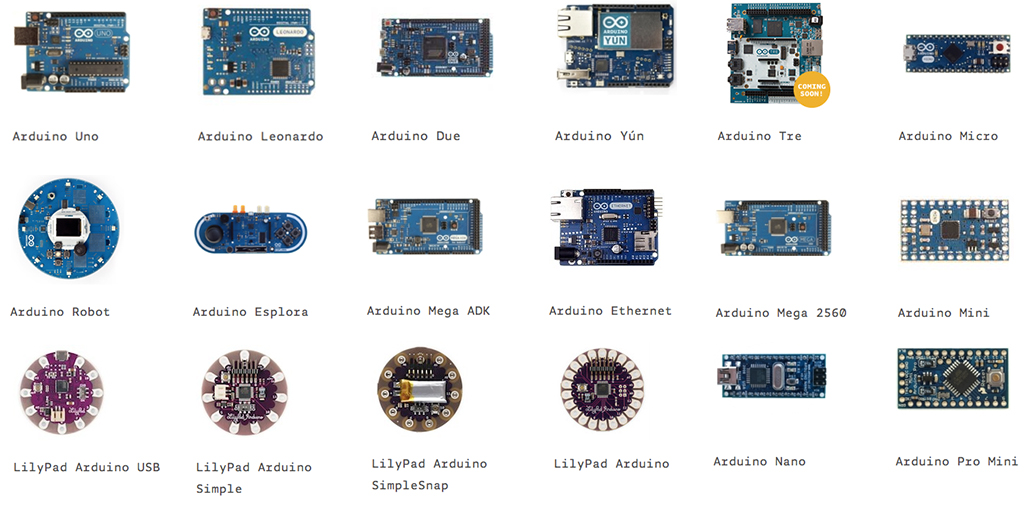
\includegraphics[width=0.9\linewidth]{ArduinoFamily}
	\caption[Arduino család néhány fajtája]{Arduino család néhány fajtája}
	\label{fig-arduinofamily}
\end{figure}
\subsection{Arduino Nano}
Elsősorban UNO-val\cite{arduinouno} terveztem elkészíteni ezt a projektet, de helyszűkében kénytelen voltam egy kisebb mikrokontroller után kutatni. Ekkor esett a választásom az Arduino Nano-ra\cite{arduinonano}. Az Arduino Nano az Arduino UNO kompaktabb változata, mely ugyanazt az ATmega328 mikrovezérlőt használja, így teljesítményében és képességeiben nagyon hasonló az UNO-hoz. A mikrovezérlő tartalmaz:
\begin{itemize}
	\item Processzort
	\item Memóriát
	\item Perifériákat:
	\begin{itemize}
		\item Időzítő áramkörök
		\item Analóg és digitális be- és kimenetek
		\item Kommunikációs interfészek (UART, SPI, I2C) és egyéb funkciók
	\end{itemize}
\end{itemize}

\begin{figure}[th!]
	\centering
	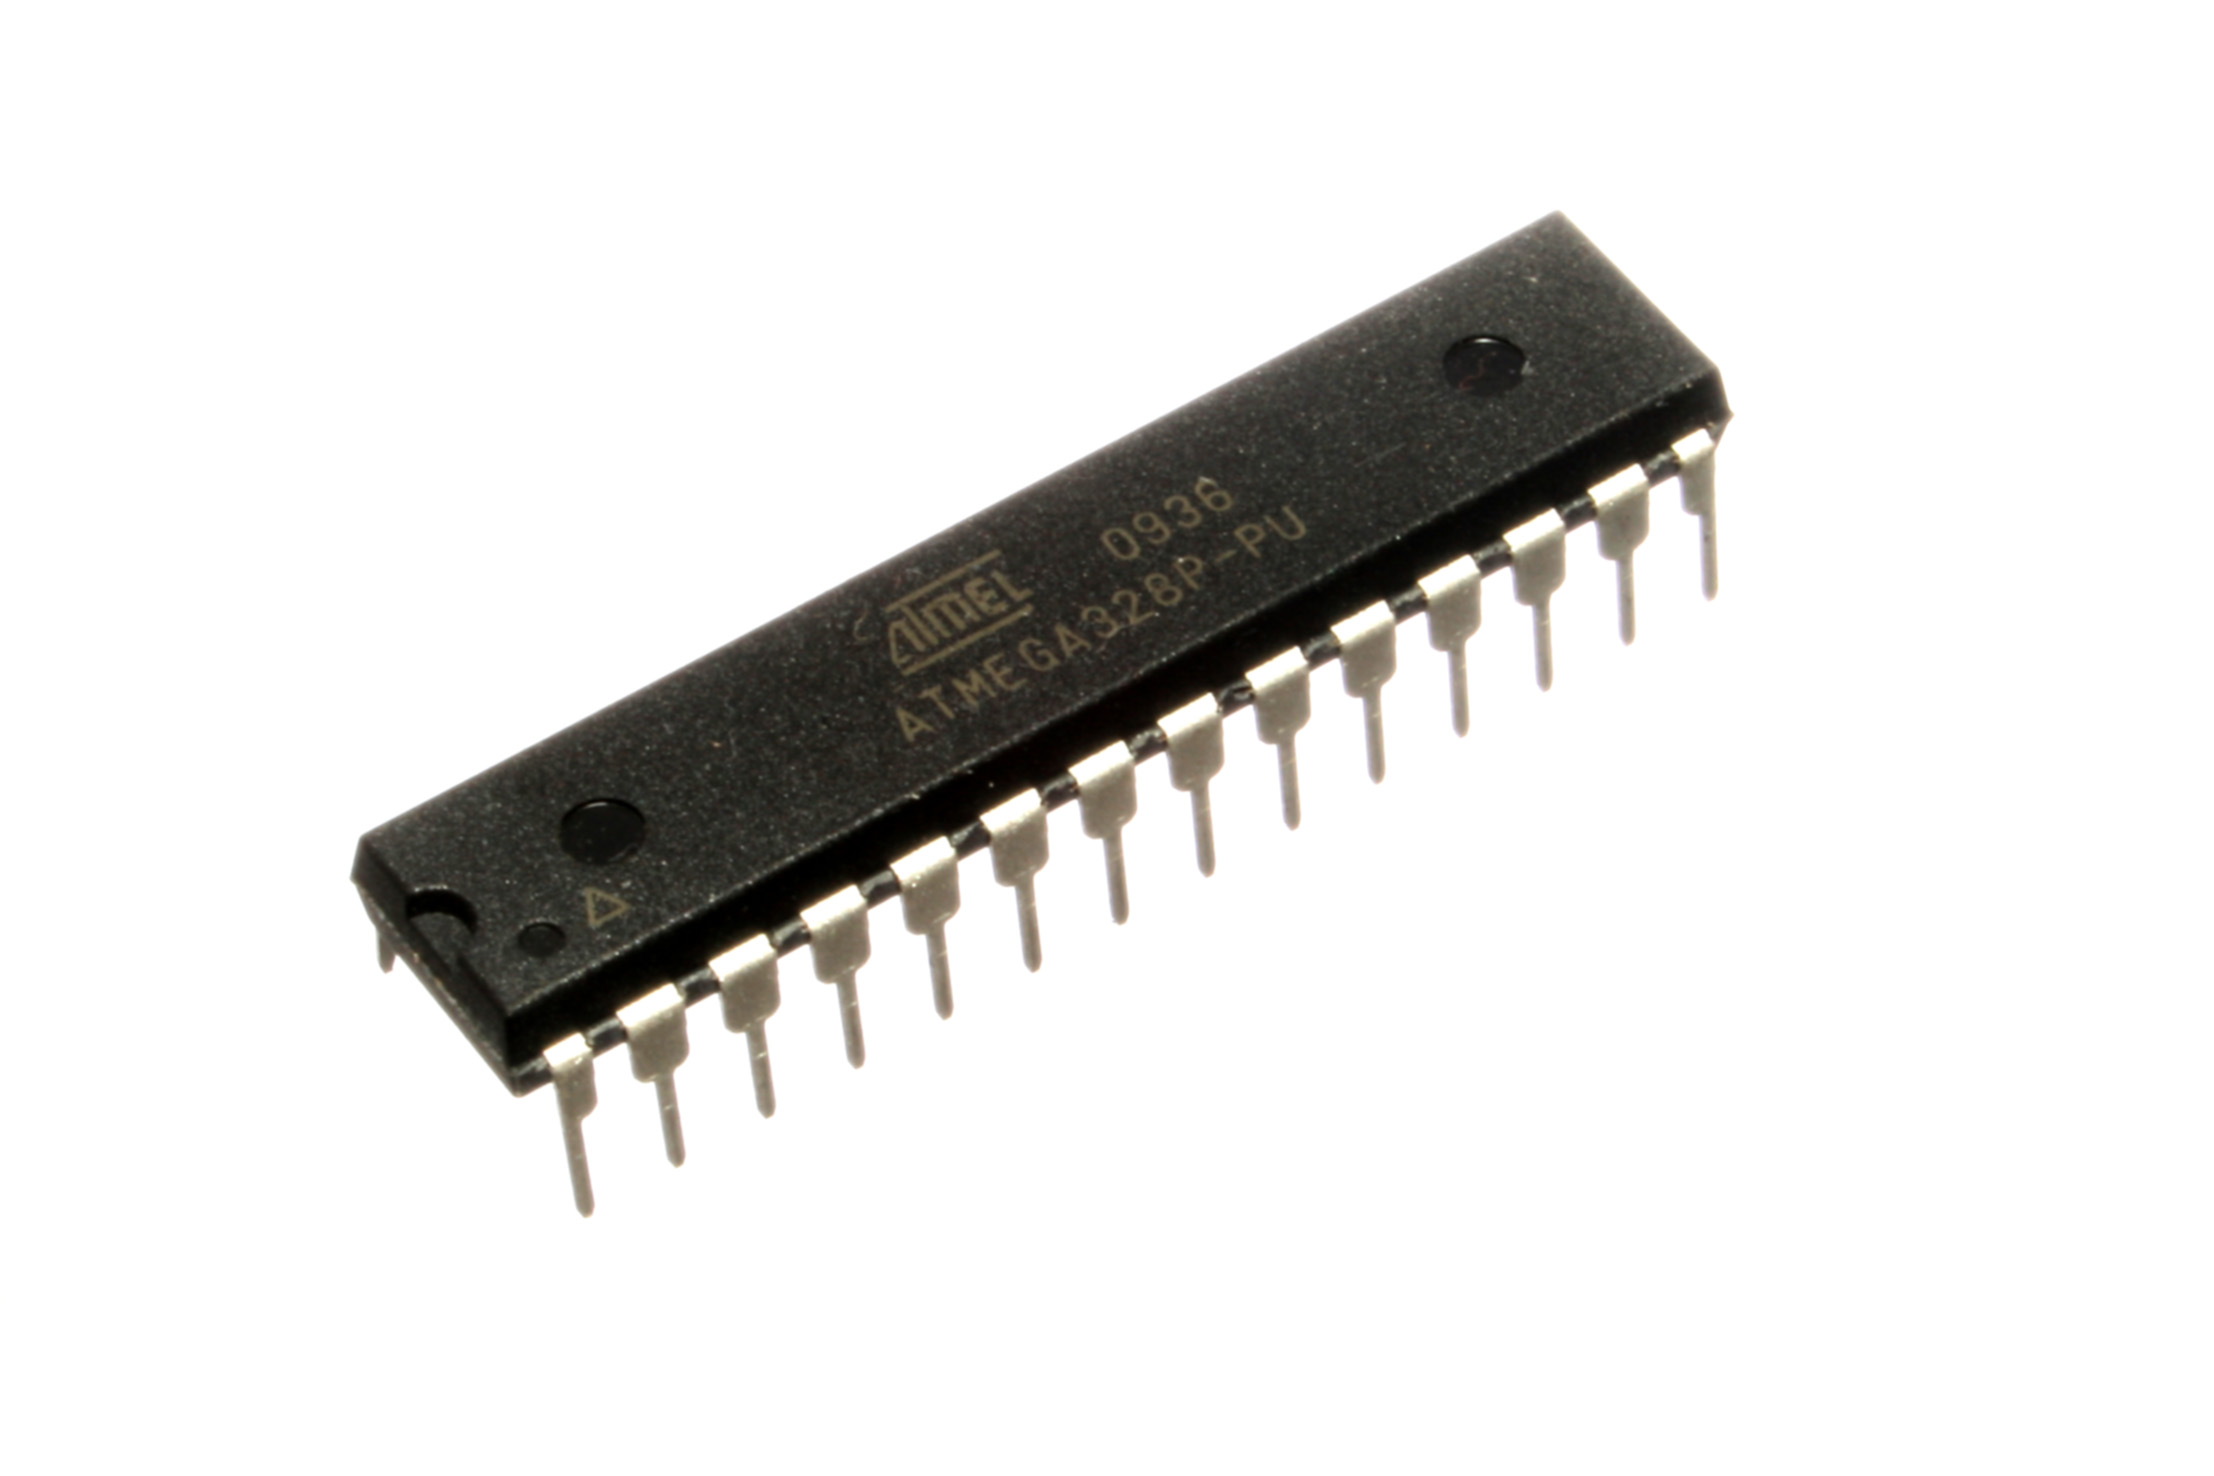
\includegraphics[width=0.4\linewidth]{ATMEGA328P-PU}
	\caption[ATmega328P]{ATmega328P mikrovezérlő}
	\label{fig:atmega328p-pu}
\end{figure}

Ezek segítségével tudunk szenzorjeleket mérni, nyomógombok vagy más beviteli eszközök állapotát beolvasni. A Nano áramköri lap szerepe az, hogy a mikrovezérlő lábait kivezesse. Így kényelmesebben és egyszerűbben rá tudjuk kötni a különböző eszközöket, amiket vezérelni szeretnénk, vagy értékeket beolvasni róluk. 

A mikrokontrollereken általában nem fut operációs rendszer, ezért minden erőforrást a feladatra összpontosít és egy garantált maximális idő alatt képes végre hajtani a feladatokat. 

Ahhoz hogy külső eszközöket és áramköröket rátudjunk csatlakoztatni, ismernünk kell a Nano lábkiosztását, amikre a kódból tudunk hivatkozni és vezérelni őket, áramköri lapon fel van tüntetve, hogy melyik lábat melyik számmal érjük el.  A Nano-n 14 digitális ki- és bemenet található (D0–D13), valamint 8 analóg bemenet (A0–A7), melyek közül az A0–A5 lábak digitális bemenetként és kimenetként is használhatók. A Nano-n található továbbá fix 3.3,V és 5,V-os kimeneti feszültségű láb is. Ez a lábkiosztás látható \aref{fig:arduino-nano-pinout}. számű ábrán.

\begin{figure}[th!]
	\centering
	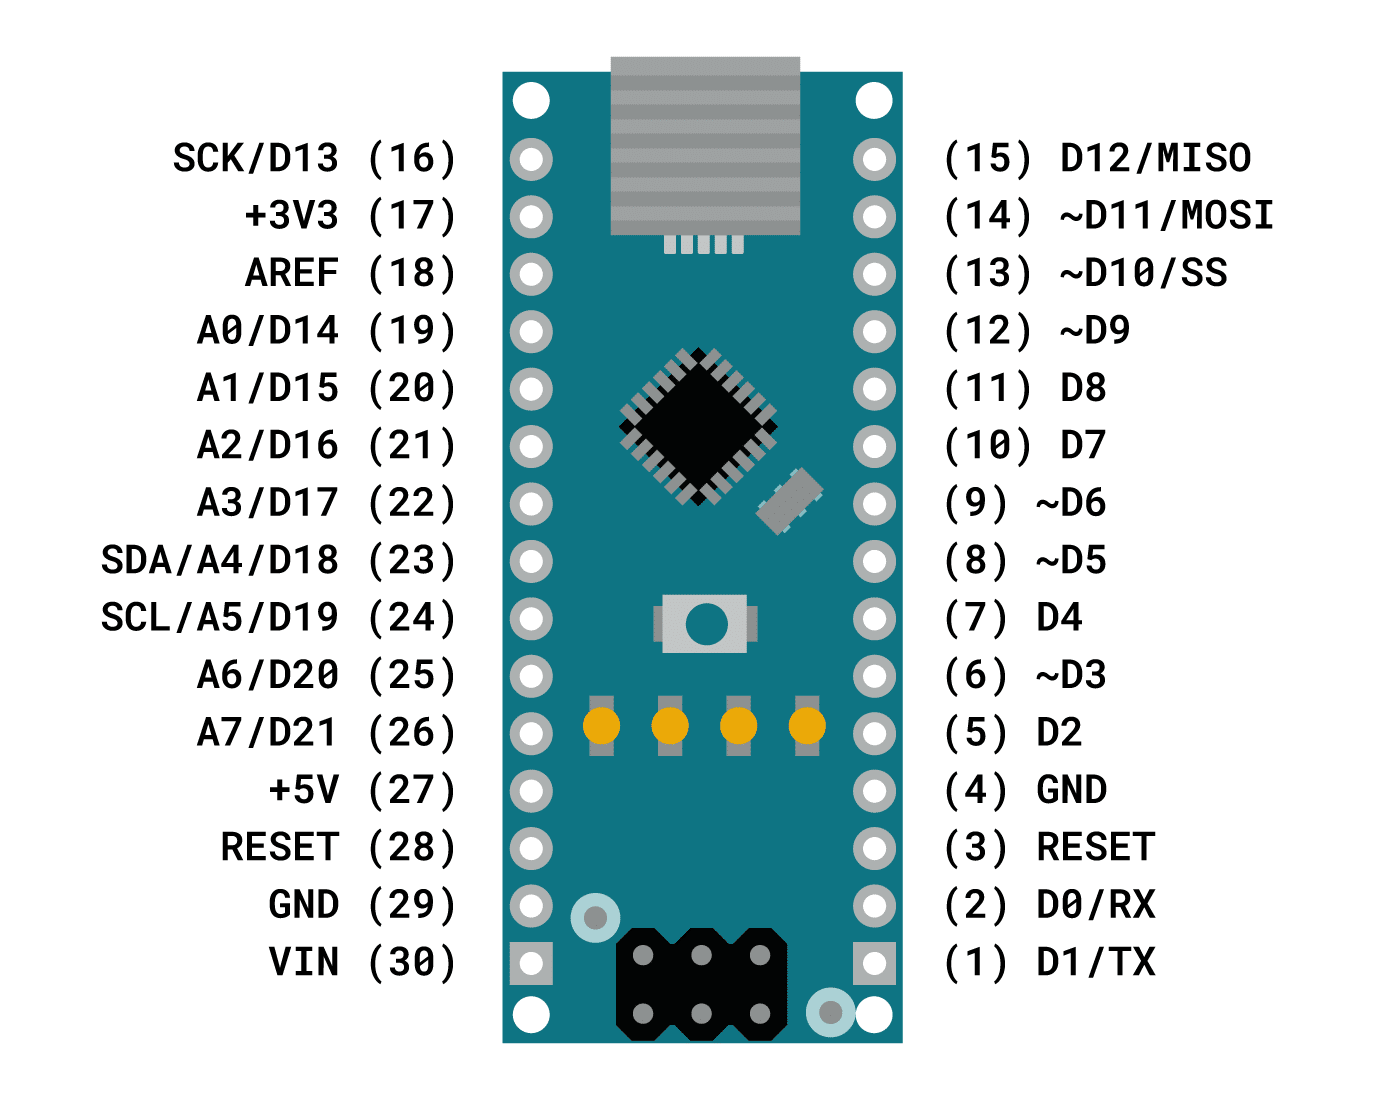
\includegraphics[width=0.7\linewidth]{arduino-nano-pinout}
	\caption[Nano felépítés]{Arduino Nano lábkiosztása}
	\label{fig:arduino-nano-pinout}
\end{figure}

\subsection{Miért választottam az Arduino Nano-t?}
Szakdolgozatom során az Arduino Nano-t választottam, mivel több olyan előnye van, amelyek különösen fontosak a projektem szempontjából:

\begin{itemize}
	\item \textbf{1. Kompakt méret.} A Nano mérete kisebb, mint az UNO-é, így ideális választás volt, mivel helyszűkében voltam.
	\item \textbf{2. Egyszerű használat és támogatottság.} Az Arduino Nano széles körben elterjedt mikrokontroller, amelyhez könnyen elérhetőek könyvtárak és példakódok, ezzel egyszerűsítve a fejlesztést.
	\item \textbf{3. Megfelelő teljesítmény és elegendő számú I/O port.} A Nano szintén ATmega328 mikrovezérlőt használ, amely tökéletesen megfelel az ADNS-9800 szenzor kezelésére, a szenzor mozgatására, valamint az adatok továbbítására.
	\item \textbf{4. Megbízhatóság és stabilitás.} A stabil működés létfontosságú, mivel a projektem dokumentumok folyamatos szkennelését, adatgyűjtést és adatátvitelt igényel hosszabb ideig.
	\item \textbf{5. Költséghatékonyság.} Az Arduino Nano az egyik legkedvezőbb árú fejlesztőeszköz, amely tökéletesen kielégíti a projekt követelményeit.
	\item \textbf{6. Egyszerű programozhatóság és csatlakoztatás.} Az Arduino Nano könnyen programozható az Arduino IDE használatával, programokat egyszerűen USB-n keresztül tölthetünk fel rá.
\end{itemize}
\subsection{Az Arduino alkalmazási területei}
\begin{itemize}
	\item \textbf{Kezdő projektekhez.} Az Arduino Board-ok tökéletesek a kezdők számára akik az elektronikát és az informatikát szeretnék ötvözni. A fejlesztő környezetet egyszerű kezelni, valamint a könyvtárak és a példa kódok is nagyon sokat segítenek azoknak az embereknek akik elkezdenek érdeklődni az ilyen dolgok iránt.
	\item \textbf{Oktatási platform.} Könnyen kezelhetősége miatt szokták alkalmazni, hogy ezekkel az eszközökkel tanítsák meg az elektronika és az informatika működését.
	\item \textbf{Robotikában.} A nagy vállalatok vezetői is felfedezték ezt a technológiát, és gyakran Arduino Board-okat használnak a robotok megvalósításához és vezérléséhez.
	\item \textbf{Zene és művészet.} Az Arduino Board-okat szokták egyszerű hangszerek létrehozására is alkalmazni, vagy már meglévő hangszerekbe beépíteni elektronikus alkatrészként.
	\item \textbf{IoT - Internet of Things.} Legtöbb esetben okos otthon rendszerekbe szokták beépíteni, mert sok szenzort rá tudunk csatlakoztatni amikkel könnyen vezérelhetjük a saját otthonunkat. 
	\item \textbf{Viselhető eszközök. (Wearables)} Kompakt méretük miatt könnyen beépíthetőek ruhákba, akár ékszerekbe vagy más hordozható eszközökbe. Amelyekkel mozgásokra reagálhatunk mérhetünk testhőmérsékletet és még sok mást.
\end{itemize}
\section{Visual Studio}
A projekt szoftveres részét Visual Studio\cite{visual-studio} fejlesztői környezettel készítettem el, mert ez áll hozzám a legközelebb. Itt valósítottam meg az interpolációt a kép minőségvesztés nélküli növelését. Valamint a program irányító felületét is itt programoztam le. 
\section{Github}
A verziókövetéshez a Githubot\cite{github} használtam azon belül is a Github Desktop-ot, mellyel könnyen tudtam több platformon is dolgozni a projekten, valamint ha valamit elrontottam könnyen vissza tudtam állítani a projektet egy korábbi verzióra.
\chapter{Hardveres megvalósítás}
\section{ADNS-9800 szenzor}
Az általam készített szkennernek a lelke a kicsi és olcsó ADNS-9800\cite{adns9800} lézeres optikai érzékelő. Az eredeti felhasználási módja ennek az eszköznek az volt, hogy egerek mozgását kövessék. Ennek a szenzornak az a különlegessége, és azért volt megfelelő számomra, mivel úgy követi a mozgást, hogy folyamatosan képeket készít. Ezáltal fel tudtam használni a projektembe mint egy kis kamerát, valamint gyors képfeldolgozási képességgel rendelkezik, ezért alkalmas dokumentumok beolvasására. 
\subsection{Működése}
 Egy beépített lézer megvilágítja a szenzor alatt lévő felületet, majd a lencse készít egy képet. A beépített kis processzor dolgozza fel ezeket az adatokat, és számítja ki, hogy az eszköz milyen irányba mozdult el. 
\begin{figure}[th!]
	\centering
	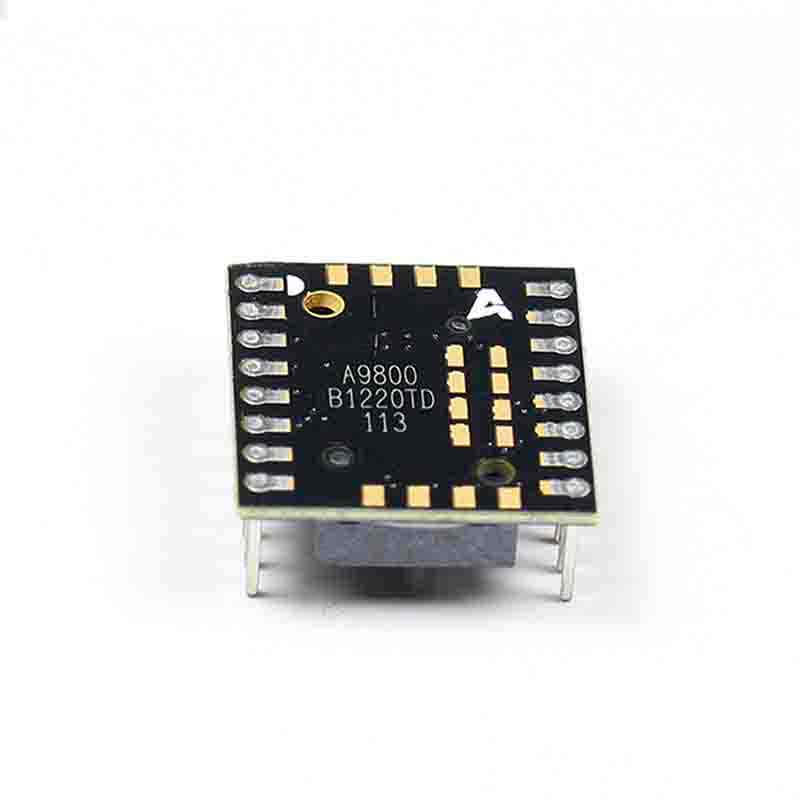
\includegraphics[width=0.4\linewidth]{ADNS9800base}
	\caption[ADNS9800]{ADNS-9800 szenzor}
	\label{fig:adns9800base}
\end{figure}

Az általam választott szenzor már nyáklappal volt ellátva így azzal nem volt teendőm. Ezáltal egyszerűbb volt a bekötése és az elhelyezése is.

\begin{figure}[th!]
	\centering
	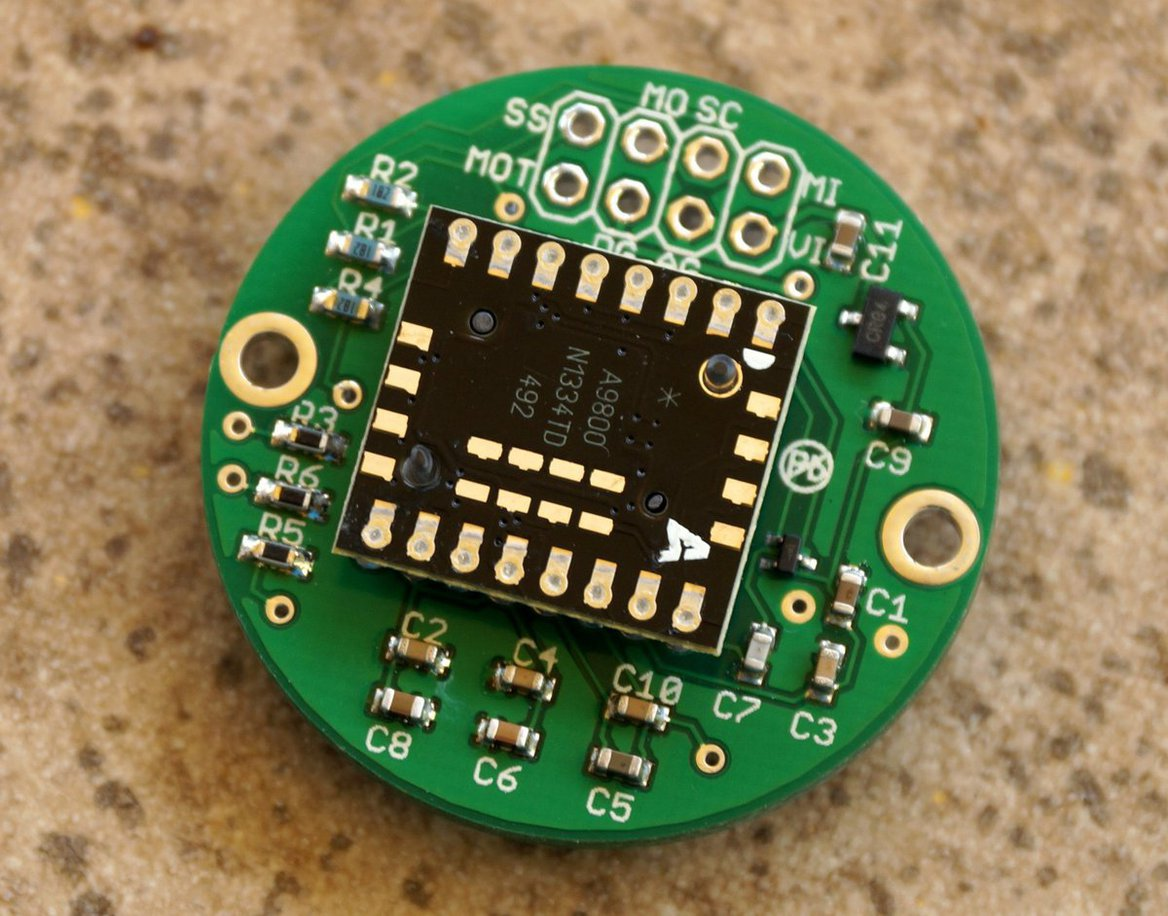
\includegraphics[width=0.5\linewidth]{ADNS9800}
	\caption[ADNS9800]{ADNS-9800 szenzor nyák lapra szerelve}
	\label{fig:adns9800}
\end{figure}

Csak egy problémám volt, hogy a nyáklappal szerelt verzió 3.3\,V-os logikai szinttel működött viszont az Arduino UNO 5\,V-os szinttel. Így be kellett szereznem egy két irányú logikai szintillesztő\cite{szintilleszto} modult ami átalakította a 3,3\,V-os  jelet 5\,V-ossá. Ehhez a projekthez egy 8 csatornás logikai szintillesztő modult használtam.

\begin{figure}[th!]
	\centering
	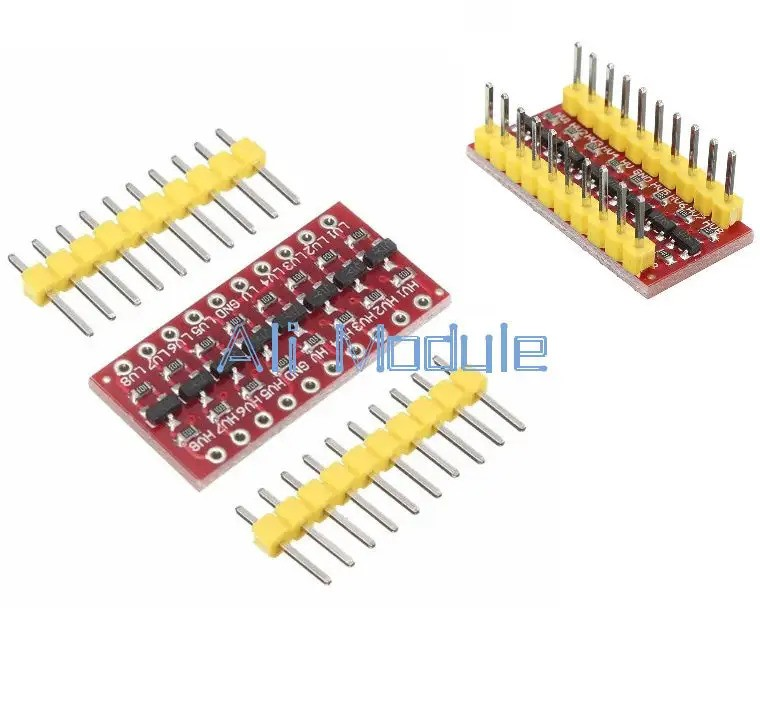
\includegraphics[width=0.6\linewidth]{szintilleszto}
	\caption[Logikai szintillesztő]{Két irányú logikai szintillesztő}
	\label{fig:szintilleszto}
\end{figure}
\pagebreak
\subsection{Adatok beolvasása}
Az adatok beolvasása közben a szenzor egy sorokból és egy oszlopokból álló képkockát készít, amely egy 30\,x\,30-as pixel rács. Ezáltal egy dokumentum szkennelése lehet akár több ezer képkocka is.
A működése a következő lépésekből áll:
\begin{enumerate}
	\item \textbf{Feltöltjük a firmware-t a szenzorra.} Erre azért van szükség, mert enélkül a szenzor csak egy hardveres érékelő, amely a lézerrel megvilágított felületről képeket készít. Ahhoz, hogy ezt az információt feldolgozza és továbbítsa szüksége van egy vezérlőprogramra, azaz firmware-re. Ezt a firmware-t minden bekapcsolás után fel kell tölteni, mert a szenzornak nincs állandó memóriája. A firmware feltöltését \aref{upload-firmware-code}. számú metódus végzi. A regiszterek megfelelő beállítása után a firmwaret soronként továbbítja  az SPI buszon keresztül a szenzornak. Ebben a metódusban fontos az időzítés hogy a szenzor helyesen értelmezze az adatokat.
	\begin{lstlisting}[language=Arduino,label=upload-firmware-code,caption=Firmware feltöltése]
		void adns_upload_firmware(){
			adns_write_reg(REG_Configuration_IV, 0x02);	
			adns_write_reg(REG_SROM_Enable, 0xd); 
			delay(10); 
			adns_write_reg(REG_SROM_Enable, 0x8); 
			adns_com_begin();
			SPI.transfer(REG_SROM_Load_Burst | 0x80); 
			delayMicroseconds(15);
			unsigned char c;
			for(int i = 0; i < firmware_length; i++){ 
				c = (unsigned char)pgm_read_byte(firmware_data + i);
				SPI.transfer(c);
				delayMicroseconds(15); 
			}
			adns_com_end();
		}
	\end{lstlisting}
	%%talán bele lehetne vinni a winforms-os elindítást
	\clearpage
	\item Majd a \textbf{sendFrame()} metódust meghívva készítünk egy képet a szenzorral. Amit egy nagy sebességű, full--duplex kommunikációs protokollal (Serial Peripheral Interface~--~SPI) kiolvasunk és eltároljuk, ahol a kommunikáció egy órajel vezérelt mechanizmussal működik. 
	\begin{lstlisting}[language=Arduino,label=sendFrame,caption=sendFrame metódus]
		void sendFrame() {
			adns_write_reg(REG_Power_Up_Reset, 0x5A);
			delay(50);
			adns_write_reg(REG_LASER_CTRL0, 0x00);
			adns_write_reg(REG_Frame_Capture,0x93);
			delayMicroseconds(120); 
			adns_write_reg(REG_Frame_Capture,0xc5);
			delayMicroseconds(120); 
			delay(1); 
			adns_com_begin(); 
			delayMicroseconds(100); 
			byte readys = 0;
			while(readys == 0){
				SPI.transfer(REG_Motion & 0x7f);
				delayMicroseconds(100); 
				readys = SPI.transfer(0); 
				readys = readys & 1;
				delayMicroseconds(20);
			}
			SPI.transfer(REG_Pixel_Burst & 0x7f); 
			delayMicroseconds(100); 
			Serial.print("FRAME:");
			for (int i = 0;i<900;i++){
				byte pixelValue = SPI.transfer(0);  
				Serial.print(pixelValue);
				Serial.print(" ");
			}
			delayMicroseconds(15); 
			adns_com_end();  
			delayMicroseconds(5); 
			Serial.println();
		}
	\end{lstlisting}
	\clearpage
	A metódus működése:
	\begin{enumerate}[label=\arabic*.]
		\item \textbf{Szenzornak kiadjuk, hogy készítsen egy képet.} Ekkor bele írjuk a megfelelő értéket a REG\_Frame\_Capture regiszterbe. A szenzor ekkor egy 30\,x\,30 pixeles képkockát olvas be.
		\item \textbf{Várunk amíg a szenzor elkészíti a képet.} Az Arduino egy ciklusban folyamatosan ellenőri a szenzor állapotát ezért amíg a szenzor nem jelzi, nem olvassuk ki az értéket.
		\item \textbf{A szenzor továbbítja a képkockát.} A Pixel Burst regiszteren keresztül történik a képkocka eljuttatása a szenzortól az Arduino-ig SPI kapcsolattal. Az SPI kapcsolat négy vezetéken keresztül történik:
		\begin{itemize}
			\item \textbf{MOSI }(Master Out, Slave In): Az adatok a mikrokontroller felől a szenzor felé mennek.
			\item \textbf{MISO }(Master In, Slave Out): Az adatok a szenzor felől mennek az Arduino felé.
			\item \textbf{SCLK }(Serial Clock): Az órajel, amelyet az Arduino generál.
			\item \textbf{CS }(Chip Select): Az adott szenzort választja ki a kommunikációhoz.
		\end{itemize}
		\item \textbf{Az Arduino továbbítja az adatokat a számítógépre.} Az adatok soros kommunikáción keresztül kerülnek a számítógépre ahol az feldolgozza ezeket. Minden képkocka ''FRAME:'' előtaggal kezdődik, amit a szenzor által olvasott színintenzitás értékek követnek. Egy példa frame sor:
		
		\verb|FRAME: 124 128 130 122 120 119 118 117 116 ...|
	\end{enumerate}
\end{enumerate}
\subsection{Szenzor mozgása}

A szenzort két motor mozgatja az egyik vízszintesen a másik pedig függőlegesen. A projekthez egy bipoláris valamint egy unipoláris léptetőmotort\cite{motorvezerlok} használtam. Mivel egy meglévő szkennerbe építettem bele az egész elektronikát, ezért a függőleges tengely mozgatására szolgáló bipoláris léptetőmotor már adott volt. Viszont a szenzor nagyon kis képet készít ezért finom mozgásokra volt szükségem, ebben segítséget nyújtott a már előre beépített fogaskerekek, amik áttétként funkcionálnak. Ezáltal a motor egy lépése jelentősen kisebb elmozdulás volt fizikailag, így jól tudtam pozicionálni. 
\begin{figure}[th!]
	\centering
	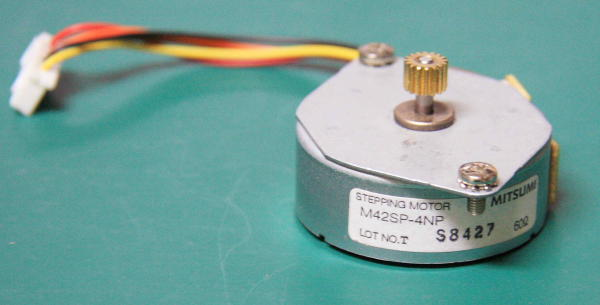
\includegraphics[width=0.4\linewidth]{MITSUMI-Stepping-Motor-M42SP-4NP}
	\caption[Mitsumi]{\footnotesize {MITSUMI M42SP-4NP bipoláris motor a függőleges mozgáshoz}}
	\label{fig:mitsumi-stepping-motor-m42sp-4np}
\end{figure}
\pagebreak

Mindkét motornál half-step vezérlési módot használtam, hogy még finomabb és pontosabb mozgást tudjak végezni velük. Ennek az a lényege, hogy a motor kétszer annyi lépésben teszi meg ugyanazt a fordulatot. Ez úgy lehetséges, hogy a négy tekercs közül először egy tekercs kap áramot, majd az első és a második egyszerre, majd csak a második, így a lépés szám a duplájára nő a szögelfordulás pedig a felére csökken.

\begin{figure}[th!]
	\centering
	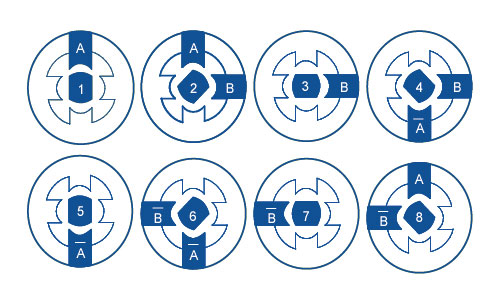
\includegraphics[width=0.7\linewidth]{stepper-motors-half-step}
	\caption[Half Step vezérlés]{Half Step vezérlés működése}
	\label{fig:stepper-motors-half-step}
\end{figure}


A vízszintes mozgáshoz beépítettem egy unipoláris léptetőmotort, amely egy ULN2003 motorvezérlő modullal működik, amit nagyon gyakran használnak ilyen kis apró finom mozgásokhoz, amire nekem is szükségem volt. Mivel ez a motor úgy van felépítve, hogy alapból áttétek vannak benne ezért azzal itt sem kellett foglalkoznom. 

\begin{figure}[th!]
	\centering
	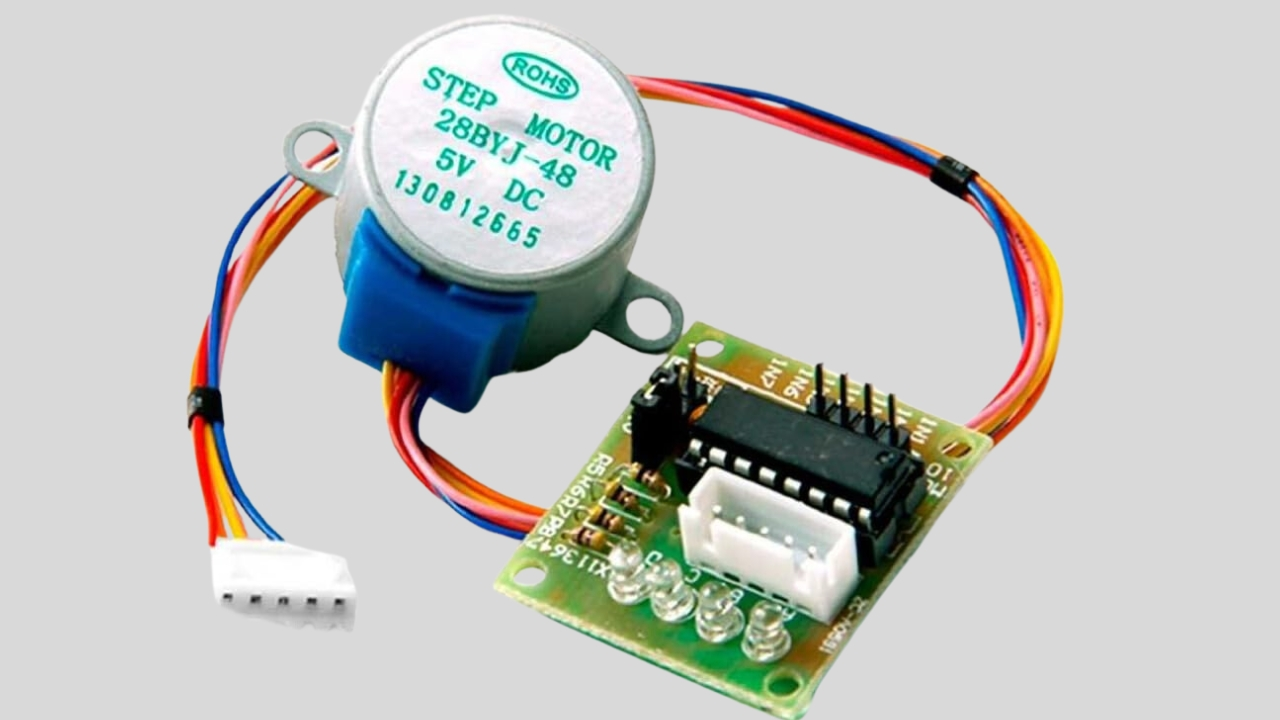
\includegraphics[width=0.5\linewidth]{28BYJ-48-modul-ULN2003}
	\caption[Unipoláris léptetőmotor]{Unipoláris léptetőmotor a vízszintes mozgáshoz}
	\label{fig:28byj-48-modul-uln2003}
\end{figure}

 A motorok egy egy bordás szíjas sínen mozognak, ezáltal a mozgás stabil lesz és csúszásmentes. Mindkettő végén van egy végállás kapcsoló, ha a vízszintes sor a végére ér ezt aktiválja és lentebb megy egy sort, valamint vissza megy a sor elejére a szenzor. Ekkor küldd az Arduino egy ''NEW\_ROW'' kulcsszót a Serial porton a számítógép felé, ezzel jelezve a feldolgozó szoftvernek, hogy új sor következik az olvasásban. Ha pedig a függőleges végálláskapcsoló válik aktívvá akkor pedig az ''END'' kulcsszót küldi el a számítógép felé, jelezve, hogy vége a dokumentumnak és vissza tér a kezdeti állásba.

\section{Hardveres bekötés}
\begin{figure}[th!]
	\centering
	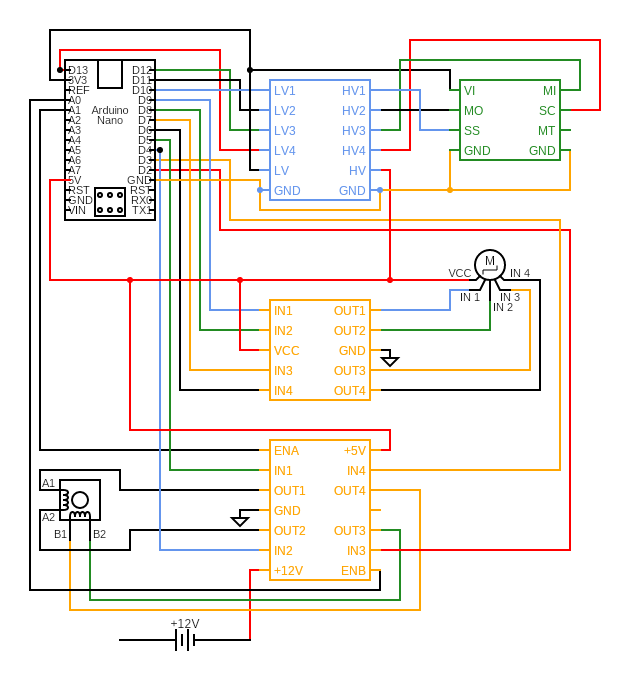
\includegraphics[width=0.7\linewidth]{circuit}
	\caption[Hardveres bekötés]{Hardveres bekötés}
	\label{fig:circuit}
\end{figure}

Már kész csak nem biztos hogy jó
\chapter{Szoftveres megvalósítás}

%%\section{Felhasznált algoritmusok/metódusok}
%%\section{Beolvasott értékek tárolása 2 dimenzós mátrixban}
%%adatszeerkezet amiben a beolvasott képet tároljuk
%%\section{Bikubik interpoláció}
%%\subsection{Működése}
%%Működésének alapjai, Matematikai leírása
%%\section{Mátrix átalakítása képpé}

\section{Az alap változók}
A feldolgozó szoftver Serial porton kapja meg az adatokat az Arduino-tól. Van két darab konstans értékem az egyik a beérkező képkocka szélessége a másik pedig a magassága, mivel a beérkező képkocka 30\,x\,30 pixel ezért ez a két érték 30. Van egy buffer-em ahol a Serial porton beérkező adatokat tárolom, erre azért van szükség mert nem biztos, hogy egy sor át tud jönni egyszerre. Valamint van egy Bicubic osztály példányom amivel a Bikubik interpolációt végzem. Végül van egy row és egy column változóm ami annak segítségére szolgál, hogy összerakjam a képkockákat egy nagy dokumentummá. Ezt a nagy dokumentumot tartalmazza a listGrid nevű változó, ami egy lista amiben listák vannak amiben egész típusú tömbök vannak. 
\begin{lstlisting}[language=CSharp]
private SerialPort serialPort;
private const int FrameWidth = 30; 
private const int FrameHeight = 30; 
private StringBuilder buffer = new StringBuilder(); 
private Bicubic resizer = new Bicubic(FrameWidth, FrameHeight, 2);

int row = 0;
int column = 0;

private List<List<int[]>> listGrid = new List<List<int[]>>();
\end{lstlisting}

\section{Inicializáló metódusok}
Van egy soros portot beállító metódus. Aminek segítségével megnyitom a soros portot és beállítom a megfelelő BaudRate-t. Jelen esetben 115200 bit/másodperc. Hozzárendelem a serialPort változó DataReceived eseményéhez a saját metódusomat, ami azt jelenti, hogy amikor érkezik adat a soros porton akkor meghívja azt a metódust. Ezután megnyitom a soros portot hogy tudjam olvasni az adatokat róla, és írok egy ''reset'' kulcsszót az Arduino felé ezen a porton keresztül, hogy alaphelyzetbe tegyem a szenzort.
\begin{lstlisting}[language=CSharp]
	private void InitializeSerialPort()
	{
		serialPort = new SerialPort("COM3", 115200);
		serialPort.DataReceived += SerialPort_DataReceived;
		serialPort.Open();
		serialPort.Write("reset");
	}
\end{lstlisting}

\chapter*{Összegzés}
Tapasztalatok amiket szereztem a projekt megvalósítása közben
Tovabbfejlesztési gondolatok

színes vagy szürke képet szeretne beolvasni
soros porton küldok egy bitet hogy színes vagy szürke legyen a kép a studiobol
felbontásra vonatkozóan például  feles átfedéssel 
\addcontentsline{toc}{chapter}{Összegzés}
\chapter*{Források}
\begin{itemize}
	\item \ref{fig-arduinofamily}. ábra: \emph{\url{https://predictabledesigns.com/wp-content/uploads/2017/10/HeroImage.png}}
	\item \ref{fig:atmega328p-pu}. ábra: \emph{\url{https://techfun.hu/wp-content/uploads/2017/09/11.jpg}}
	\item \ref{fig:arduino-nano-pinout}. ábra: \emph{\url{https://www.makerguides.com/wp-content/uploads/2020/10/arduino-nano-pinout-768x603.png}}
	\item \ref{fig:adns9800base}. ábra: \emph{\url{https://www.sicstock.com/cdn/shop/products/551554.jpg?v=1544514465}}
	\item \ref{fig:szintilleszto}. ábra: \emph{\url{https://www.elektrobot.hu/items/3607_1.webp}}
	\item \ref{fig:mitsumi-stepping-motor-m42sp-4np}. ábra: \emph{\url{https://www.picmicrolab.com/wp-content/uploads/2014/04/MITSUMI-Stepping-Motor-M42SP-4NP.jpg}}
	\item \ref{fig:stepper-motors-half-step}. ábra: \emph{\url{https://www.orientalmotor.com/images/stepper-motors/stepper-motors-half-step.jpg}}
	\item \ref{fig:28byj-48-modul-uln2003}. ábra: \emph{\url{https://www.hwlibre.com/wp-content/uploads/2024/10/28byj-48-circuito.jpg}}
\end{itemize}


\begin{thebibliography}{8}
\addcontentsline{toc}{chapter}{\bibname}
\bibitem{arduino} Arduino: \url{https://www.arduino.cc/en/Guide/Introduction}
\bibitem{whatisanarduino} What is an Arduino: \url{https://learn.sparkfun.com/tutorials/what-is-an-arduino/all}
\bibitem{arduinouno} Arduino UNO: \url{http://dx.doi.org/10.6084/m9.figshare.11971794.v1}
\bibitem{arduinonano} Arduino Nano: \url{https://docs.arduino.cc/hardware/nano/}
\bibitem{visual-studio} Microsoft Visual Studio: \url{https://visualstudio.microsoft.com/}
\bibitem{github} Github: \url{https://github.com/}
\bibitem{adns9800} ADNS-9800 adatlap:\url{https://datasheet.octopart.com/ADNS-9800-Avago-datasheet-10666463.pdf}
\bibitem{adns9800_buy} ADNS-9800 vásárlás: \url{https://www.tindie.com/products/citizenjoe/adns-9800-motion-sensor/}
\bibitem{adns9800_2} ADNS-9800 tutorial get travel distance: \url{https://www.instructables.com/Arduino-Tutorial-ADNS-9800-Laser-Mouse-Traveled-Di/}
\bibitem{adns9800_3} ADNS-9800 5\,V mód aktiválása: \url{https://forum.arduino.cc/t/using-avago-adns9800/292172/2}
\bibitem{szintilleszto} Logikai szintillesztő modul: \url{https://www.elektrobot.hu/termek.php?filename=3607.html&i=3607}
\bibitem{motorvezerlok} Léptető motorok: \url{https://docs.arduino.cc/learn/electronics/stepper-motors/}
\bibitem{bicubic_video} Bicubic Interpolation by Computerphile: \url{https://www.youtube.com/watch?v=poY_nGzEEWM}
\bibitem{bicubic_wikipedia} Bicubic Interpolation from wikipedia: \url{https://en.wikipedia.org/wiki/Bicubic_interpolation}
\bibitem{catmull-rom_spline} Catmull-Rom Spline: \url{https://en.wikipedia.org/wiki/Centripetal_Catmull%E2%80%93Rom_spline}
\bibitem{image_upscale} Kép nagyítás Bikubik interpolációval: \url{https://medium.com/@amanrao032/image-upscaling-using-bicubic-interpolation-ddb37295df0}
\end{thebibliography}

% Aláírt, szkennelt nyilatkozat beillesztése a szakdolgozat végére
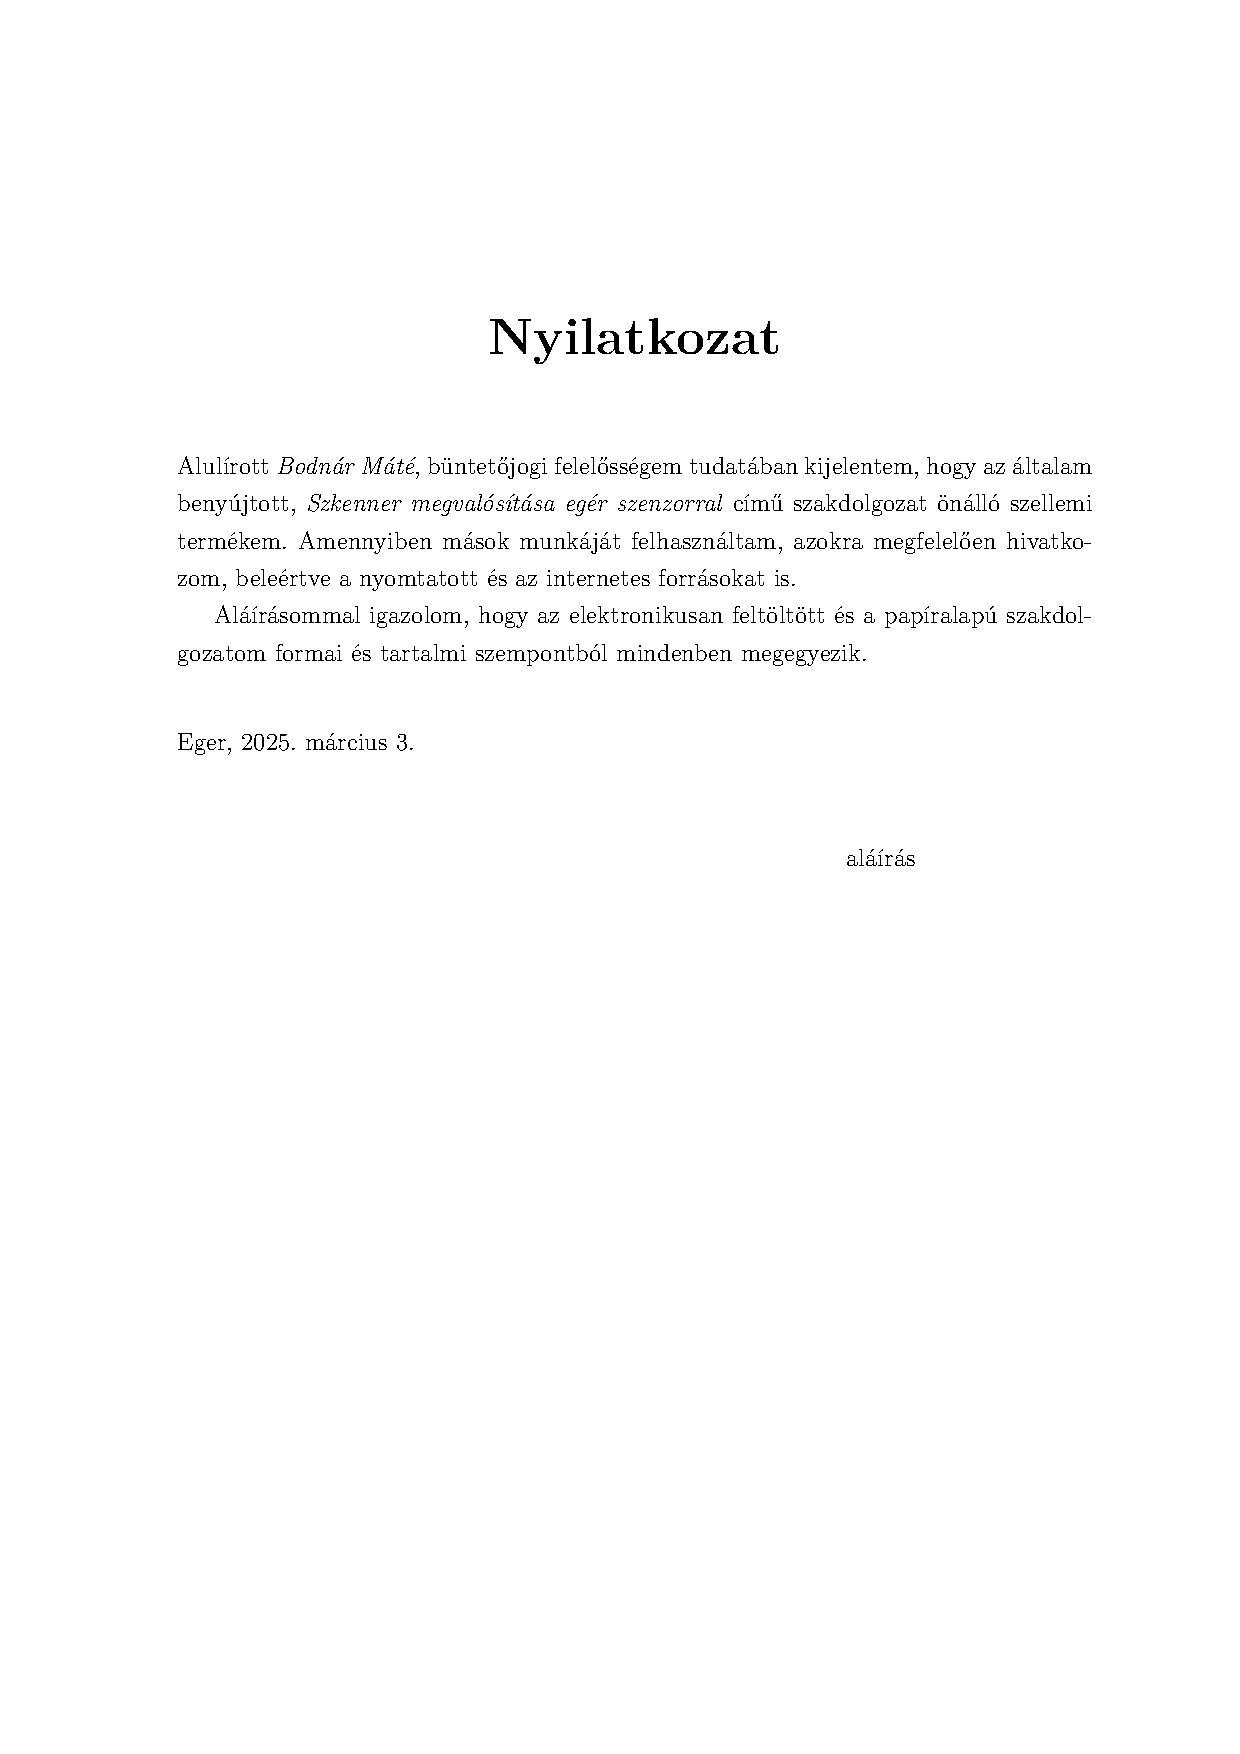
\includepdf{nyilatkozat.pdf}

\end{document}
